%TODO: ARREGLAR EJERCICIO 1B
\documentclass{article}
\usepackage[utf8]{inputenc}
\usepackage[spanish]{babel}
\usepackage{graphicx, graphics, float, hyperref}
\usepackage{listings}
\usepackage[a4paper, total={6in, 10in}]{geometry}

\title{SSO Práctica 1 Sesión 3}
\author{Andrés Merlo Trujillo}
\date{}
\hypersetup{
    colorlinks=true,
    linkcolor=black,
}

\begin{document}

\maketitle

\tableofcontents

\newpage
%\addcontentsline{toc}{section}{Ejercicio 1}
%\section*{Ejercicio 1}
%\begin{figure}[H]
%    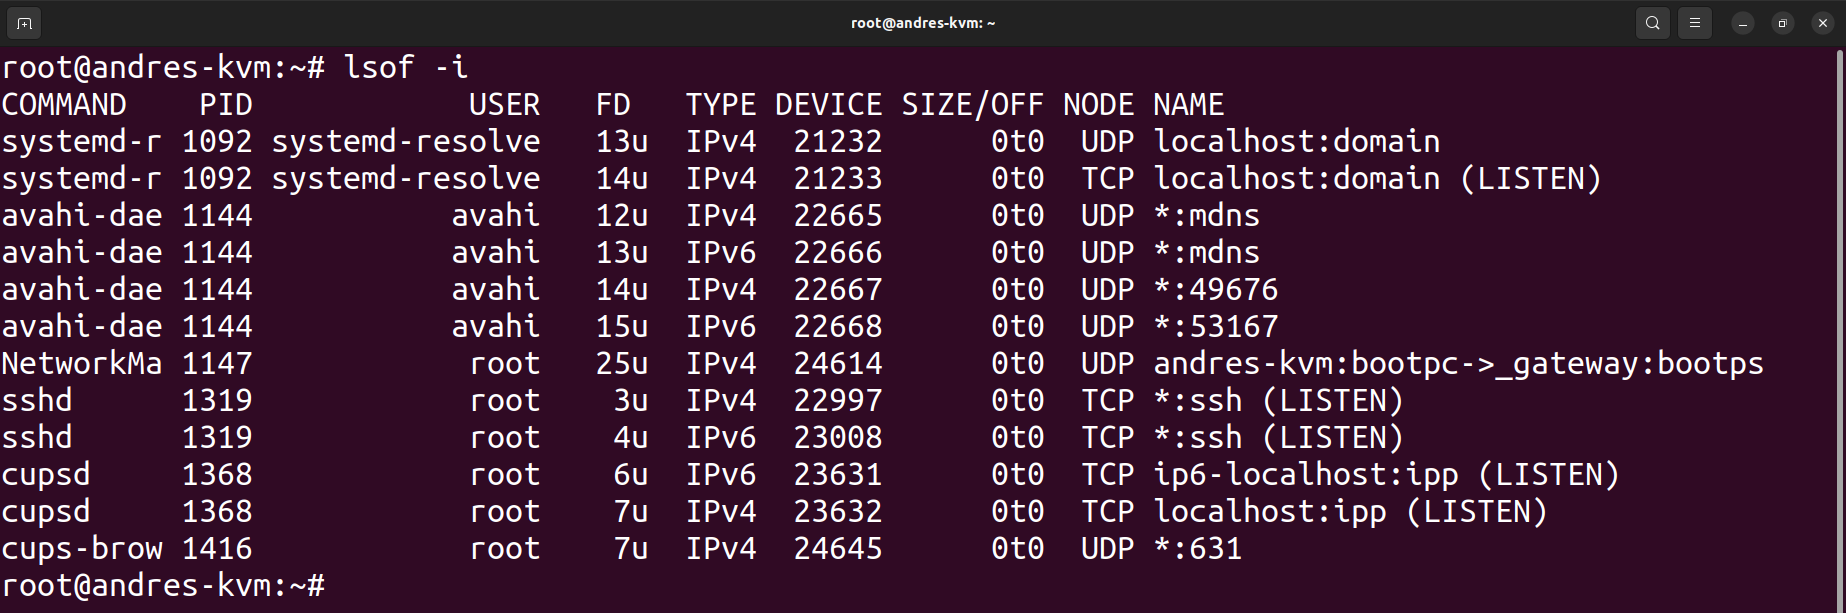
\includegraphics[width=\textwidth]{imagenes/lsofi.png}
%\end{figure}

\addcontentsline{toc}{section}{Ejercicio 1}
\section*{Ejercicio 1}

\addcontentsline{toc}{subsection}{Apartado A}
\subsection*{Apartado A}

Para crear las claves personales es necesario ejecutar la orden \verb|gpg --gen-key|. Ahora pedirá una serie de información que es necesario rellenar como el nombre o el correo.

%foto de nombre y apellidos.

A continuación aparece un sumario de los datos rellenados y al aceptarlos aparece un cuador de texto para introducir la contraseña. A continuacion pide al usuario realizar diversas cosas para generar entropia y que la clave sea lo mas aleatoria posible como mover el raton, realizar actividad de red y de disco, etc.

%foto de toda la traza.

Y ahora para mostrar las claves publicas se utiliza el comando \verb|gpg --list-keys|:

%foto de list keys

Y para mostrar las claves privadas se utiliza el comando \verb|gpg --list-secret-keys|:

%foto de list secret keys

\addcontentsline{toc}{subsection}{Apartado B}
\subsection*{Apartado B}

Primero voy a crear un archivo de texto cualquiera como el siguiente:

%foto del contenido del archivo


Y ahora para cifrar el archivo se utiliza el comando \verb|gpg --armor --recipient correo --encrypt file|. Para ello, en la parte de ``recipient'' es necesairo poner el correo que se haya usado para crear las claves en el ejercicio anterior.

Esto generara un fichero con la extension ``.asc'' el cual, si se abre, contiene lo siguiente:

%foto de la encriptacion.

Por ultimo, para descifrar el mensaje se utiliza la orden \verb|gpg --decrypt prueba.asc|, se pedira la contraseña que se inserto al crear las claves.

%foto de pedir clave


%foto de la salida del comando.

\addcontentsline{toc}{subsection}{Apartado C}
\subsection*{Apartado C}

Me he juntado con el compañero \dots \textbf{RELLENAR AQUI ESTO} para mandarnos archivos cifrados a cada uno. Para que él pueda obtener mi clave publica, la he subido a \url{https://keyserver.ubuntu.com/}.

He creado el siguiente archivo para mi compañero:

%foto del archivo 

Y con la orden \verb|gpg --armor --recipient correo --encrypt file| se encripta y se puede mandar el archivo con extension ``.asc'' sin problema.



Ahora, con el archivo cifrado de mi compañero, usando la orden \verb|gpg --decrypt file| se puede abrir.

%foto de la salida.


\addcontentsline{toc}{section}{Ejercicio 2}
\section*{Ejercicio 2}
\end{document}

%\begin{figure}[H]
%    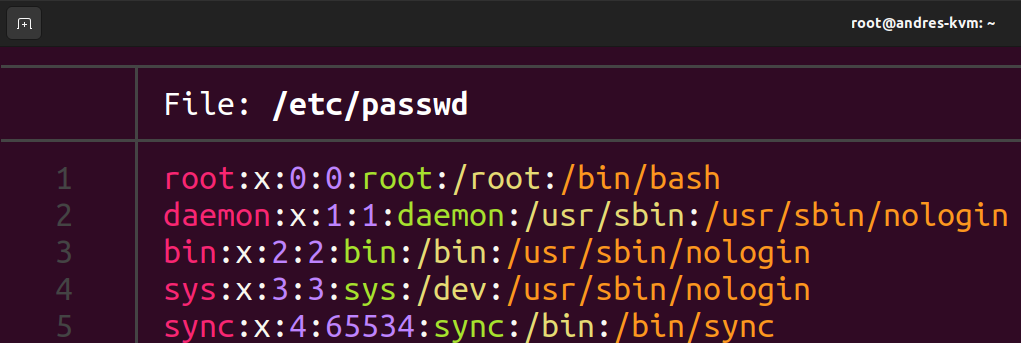
\includegraphics[width=\textwidth]{imagenes/passwdfile.png}
%    \caption{Ejemplo de entradas en el archivo.}
%\end{figure}